\chapter{Materials}
\section{Allgemeines}
Als Datensatz wurde der BrainTumour-Datensatz der Medical Segmentation Decathlon Challenge von 2018 (\cite{Antonelli.2021}) verwendet. Dieser besteht aus 750 MRT-Scans von Patienten die entweder mit einem Glioblastom oder einem niedriggradiges Gliom, also einem Hirntumor, diagnostiziert wurden. Die Bilder enthalten vier MRT-Sequenzen. Die Daten stammen von 19 verschiedenen Institutionen und wurden mit unterschiedlichem Equipment und Aufnahmeprotokollen aufgezeichnet. Die Scans wurden durch Experten der Neuroradiologie mit ihren Labels versehen.

\begin{table}[H]
\center
\begin{tabular}{|c|c|}
\hline 
Label & Bezeichnung \\ 
\hline 
0 & Background \\ 
\hline 
1 & Edema  \\ 
\hline 
2 & non-enhancing tumour \\ 
\hline 
3 & enhancing tumour \\ 
\hline 

\end{tabular} 
\caption {Label des Datensatzes}
\end{table}

Die Bilder haben eine Höhe und Breite von 240 Pixeln und eine Tiefe von 155. Durch die 4 Modalitäten hat ein Datensatz also die Form 4x240x240x155. Bis auf die Modalitäten gilt dasselbe für die Label, welche daher eine Form von 1x240x240x155 haben.

\begin{figure}[H]
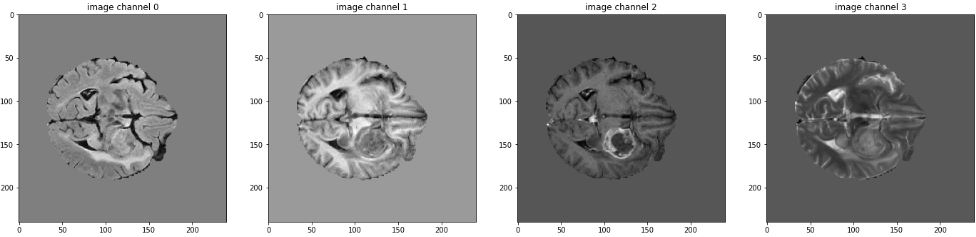
\includegraphics[width=\linewidth]{./images/DatenImg.jpg}
\captionof{figure}{Beispiel Bilddaten}
\end{figure}

\begin{figure}[H]
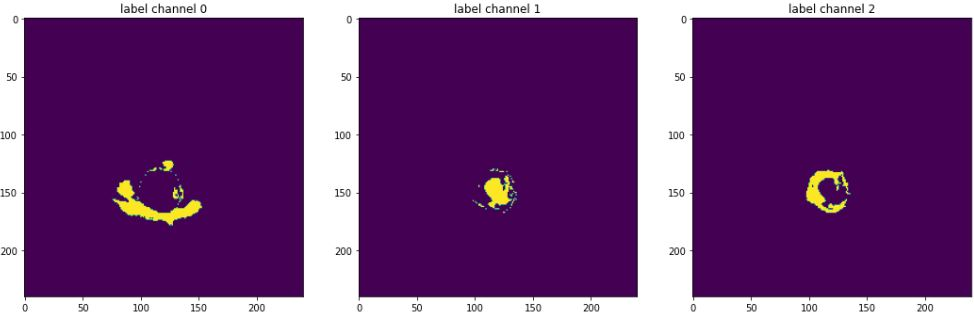
\includegraphics[width=\linewidth]{./images/DatenLabel.jpg}
\captionof{figure}{Beispiel Label (1 Channel pro Label)}
\end{figure}

\section{Verwendung des Datensatzes}
\label{Usage}
Die Daten im originalen Datensatz sind folgendermaßen aufgeteilt:
\begin{itemize}
\item Anzahl Trainingsdaten: 484
\item Anzahl Testdaten: 266
\end{itemize}

Um die Daten am Ende jedoch sinnvoll evaluieren zu können, werden auch für die Testdaten Label benötigt. Diese liegen im Original jedoch nicht vor. Deshalb wurde der Trainingsdatensatz, in dem Label enthalten sind, folgendermaßen aufgeteilt:

\begin{itemize}
\item Anzahl Trainingsdaten: 338 (70\%)
\item Anzahl Validierungsdaten: 97 (20\%)
\item Anzahl Testdaten: 49 (10\%)
\end{itemize}

